\documentclass[10pt]{article}

\pagestyle{empty}

\setlength{\textheight}{250mm}
\setlength{\textwidth}{180mm}
\setlength{\oddsidemargin}{-8mm}
\setlength{\topmargin}{-1.5cm}

\usepackage{amsmath}
\usepackage{amsmath}
\usepackage{amsthm}
\usepackage{psfrag}
\usepackage{graphicx}
\usepackage{bm}
\usepackage{mathrsfs}
\usepackage{icomma} % pacchetto per limitare lo spazio standard posto dopo la virgola in caso che la virgola sia tra cifre
\usepackage{amsfonts} % amplia i caratteri matematici disponibili
\usepackage{amssymb}
%\usepackage{wrapfig}
\usepackage{empheq}

\usepackage{epstopdf}
\usepackage[utf8x]{inputenc}
\usepackage{ifthen}

\usepackage[italian]{babel}
%\usepackage[latin1]{inputenc}

\usepackage{pgfplots}
\pgfplotsset{compat=1.9}

%\input{def}

%\newcommand{\kg}{\textrm{kg}}
%\newcommand{\K}{\textrm{K}}
%\newcommand{\m} {\textrm{m}}
%\newcommand{\dm}{\textrm{dm}}
%\newcommand{\cm}{\textrm{cm}}
%\newcommand{\mm}{\textrm{mm}}
%\newcommand{\s} {\textrm{s}}
%\newcommand{\N} {\textrm{N}}
%\renewcommand{\Pa}{\textrm{Pa}}
%\newtheorem{exerciseS}{Esercizio}[section]

%% ###########################################################
\def \flagSect{0} % 1    : numerazione
		  % else : niente
%\newcommand{\taitol}[1]  % stile titolo
%{
%%{\textit{#1}}
%{#1}
%}
\def \soluzione{Soluzione}
\def \partePrima{Concetti. }
\def \parteSeconda{Svolgimento. }
%\def \parteTerza{}
\newcommand{\sol}{\subsubsection*{\soluzione}}
\newcommand{\partone}{\ \ \ \ \ \textbf{\partePrima}}
\newcommand{\parttwo}{\vspace{0.2cm}\textbf{\parteSeconda}}

\ifnum\flagSect=1
\newtheorem{esercizio}{Esercizio}%[section]
\else
\newtheorem*{esercizio}{Esercizio}
\fi

\newtheorem*{teorema}{Teorema}
\newtheorem*{lemma}{Lemma}

% ###########################################################
%\def \flagSect{0} % 1    : numerazione
		  % else : niente
%\newcommand{\taitol}[1]  % stile titolo
%{
%%{\textit{#1}}
%{#1}
%}
\def \soluzione{Soluzione}
\def \partePrima{Concetti. }
\def \parteSeconda{Svolgimento. }
%\def \parteTerza{}
\newcommand{\sol}{\subsubsection*{\soluzione}}
\newcommand{\partone}{\ \ \ \ \ \textbf{\partePrima}}
\newcommand{\parttwo}{\vspace{0.2cm}\textbf{\parteSeconda}}

\ifnum\flagSect=1
\newtheorem{esercizio}{Esercizio}%[section]
\else
\newtheorem*{esercizio}{Esercizio}
\fi

\newtheorem*{teorema}{Teorema}
\newtheorem*{lemma}{Lemma}

% ###########################################################
%\def \flagSect{0} % 1    : numerazione
		  % else : niente
%\newcommand{\taitol}[1]  % stile titolo
%{
%%{\textit{#1}}
%{#1}
%}
\def \soluzione{Soluzione}
\def \partePrima{Concetti. }
\def \parteSeconda{Svolgimento. }
%\def \parteTerza{}
\newcommand{\sol}{\subsubsection*{\soluzione}}
\newcommand{\partone}{\ \ \ \ \ \textbf{\partePrima}}
\newcommand{\parttwo}{\vspace{0.2cm}\textbf{\parteSeconda}}

\ifnum\flagSect=1
\newtheorem{esercizio}{Esercizio}%[section]
\else
\newtheorem*{esercizio}{Esercizio}
\fi

\newtheorem*{teorema}{Teorema}
\newtheorem*{lemma}{Lemma}

% ###########################################################
%\input{logicNumb}
%\newcommand{\sectionIf}[2]
%{
%   \ifthenelse{\equal{#1}{1}}
%              {\subsection{#2}}{\subsection*{#2}}
%}
% ###########################################################

%\newcommand{\sectionIf}[2]
%{
%   \ifthenelse{\equal{#1}{1}}
%              {\subsection{#2}}{\subsection*{#2}}
%}
% ###########################################################

%\newcommand{\sectionIf}[2]
%{
%   \ifthenelse{\equal{#1}{1}}
%              {\subsection{#2}}{\subsection*{#2}}
%}
% ###########################################################



\begin{document}

\begin{center}
\textbf{Esercizi per il corso di Fluidodinamica} 
\medskip
\end{center}



\noindent
\begin{tabular}{cc}
\begin{minipage}{0.60\textwidth}
\begin{exerciseS}[Effetto Coanda sul cilindro]
Un getto d'acqua ($\rho=999\ kg/m^3$) stazionario, piano e orizzontale 
viene indirizzato su un cilindro, lambendone la superficie e
venendo deviato di un angolo $\alpha =15^\circ$.
Determinare la forza agente su una porzione del cilindro di lunghezza 
pari a $H = 2\ m$, dovuta sia al getto d'acqua,
sia all'aria circostante, sapendo che:
\begin{itemize}
  \item il fluido che circonda il getto e il cilindro \`e aria in quiete a
  pressione atmosferica di $101325\ Pa$;
  \item la larghezza del getto \`e $h=2\ cm$;
  \item la portata d'acqua per unit\`a di lunghezza nel getto \`e 
  $Q = 199\ kg\ m^{-1}\ s^{-1}$.
\end{itemize}
Sufficientemente lontano dal cilindro, il profilo di velocità sulle sezioni del getto è uniforme. Illustrare tutte le ipotesi semplificative adottate nella risoluzione dell'esercizio.

($\bm{F} = 1026\ \hat{\bm{x}} - 135\ \hat{\bm{y}} \ N$)
\end{exerciseS}
\end{minipage}
&
\begin{minipage}{0.35\textwidth}
   \begin{center}
   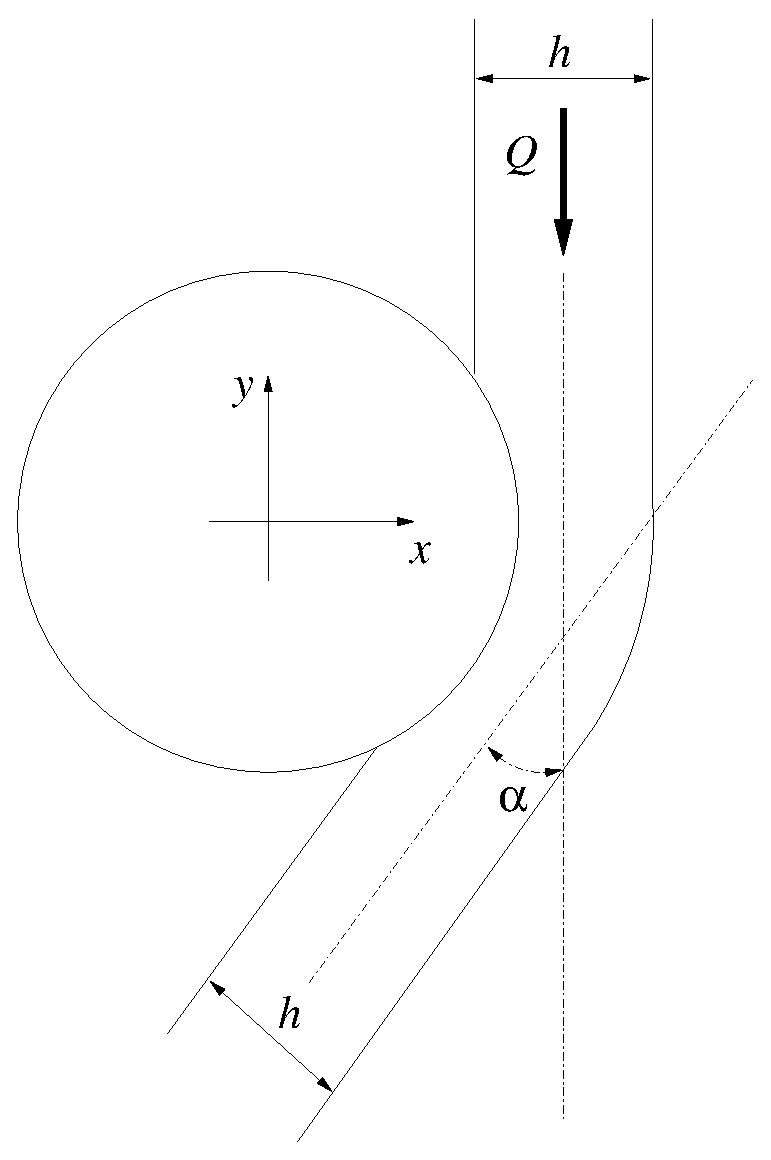
\includegraphics[width=0.90\textwidth]{./fig/coanda.eps}
   \end{center}
\end{minipage}
\end{tabular}

\vspace{1.0cm}

\sol

\partone
  Bilanci integrali di massa e quantità di moto. Equazioni di equilibrio (equazioni fondamentali della dinamica classica). Principio di azione e reazione. Integrale della normale su una superficie chiusa è identicamente nullo. Effetto Coanda (esempio della bustina da té sotto il rubinetto).

\parttwo
Vengono fatte alcune ipotesi: il problema stazionario; attorno al getto e al solido, l'aria è in quiete con pressione uniforme $p_a$; il profilo di velocità è uniforme sulle sezioni del getto considerate nelle equazioni di bilancio.

Partendo dalle equazioni di bilancio per il volume di controllo $V_{f}$ occupato dal fluido,  rielaborando il termine degli sforzi di superficie sforzi di superficie, si ricava la risultante $\bm{R}$ agente sul solido in funzione del flusso di quantità di moto del fluido attraverso la superficie $S_{f} = \partial V_f$.

Innanzitutto viene ricavata l'espressione della risultante $\bm{R}$ agente sul solido. 
\begin{itemize}
 \item Vengono scritte le equazioni di bilancio per il fluido, considerando il volume $V_f$
   \begin{equation}
     \begin{cases}
       \dfrac{d}{d t} \displaystyle\int_{V_f} \rho + \oint_{S_f} \rho \bm{u} \cdot \hat{\bm{n}} = 0 & \qquad \text{(massa)} \\
       \dfrac{d}{d t} \displaystyle\int_{V_f} \rho \bm{u} + \oint_{S_f} \rho \bm{u} \bm{u} \cdot \hat{\bm{n}} =
        \oint_{S_f} \bm{t_n} = 0  
%        \oint_{\partial \Omega} p \hat{\bm{n}} - \oint_{\partial \Omega} \bm{s_n} = 0  
        & \qquad \text{(quantità di moto)}  %\Rb^{ext}
      \end{cases}
    \end{equation}
 \item Viene introdotta l'ipotesi di stazionarietà del fenomeno, $\frac{d}{dt}\equiv 0$.
 La risultante degli sforzi viene scritta come somma degli sforzi di pressione e degli sforzi viscosi, 
\begin{equation}
\begin{split}
% & \Rb = \oint_{S_{cyl}}  {\bm{t}}_{\bm{n}} = 
% \oint_{S_{cyl}}  {\bm{s}}_{\bm{n}} - \oint_{S_{cyl}} p {\hat{\bm{n}}}_{cyl} \\
 & \oint_{S_f} \rho \bm{u} \bm{u} \cdot \hat{\bm{n}} 
  = \oint_{S_{f}}  {\bm{t}}_{\bm{n}} = 
 \oint_{S_{f}}  {\bm{s}}_{\bm{n}} - \oint_{S_f} p {\hat{\bm{n}}}_{f} \ .
\end{split}
\end{equation}

%\begin{equation}
%  \Rb = \oint_{S_{cyl}} \bm{t_n} = 
%  \int_{S_{ext}} \bm{t_n} + \int_{S_{c}} \bm{t_n} = 
%  - \int_{S_{ext}} p \bm{n}_{cyl} + \int_{S_{c}} \bm{t_n} = 
%\end{equation}


\item Viene manipolato il termine degli sforzi di superficie. Il contorno $S_f$ del volume fluido viene scomposto come unione della superficie a contatto con il solido $S_{fs}$, delle superfici ``laterali'' $S_{f\ell}$ (attraverso le quali non c'è flusso di quantità meccaniche, poichè $\bm{u}\cdot\bm{\hat{n}} = 0$) a contatto con l'aria in quiete e le sezioni ``di ingresso'' $S_{f,1}$ e ``di uscita'' $S_{f,2}$ sulle quali la velocità è uniforme, utilizzate per i bilanci integrali per il volume fluido. Viene indicata con $\bm{\hat{n}_f}$ la normale uscente dal volume $V_f$.
Il contorno $S_s$ del solido viene scomposto come unione della superficie a contatto con il fluido $S_{sf}$ e della superficie $S_{s\ell}$ a contatto con l'aria in quiete. Viene indicata con $\bm{\hat{n}_s}$ la normale uscente dal volume $V_s$.
In questo modo, la superficie $S_{fs}$ coincide con la superficie $S_{sf}$, a meno della normale invertita, $\bm{\hat{n}_f} = \bm{\hat{n}_s}$. Su queste superfici, per il terzo principio della dinamica, lo sforzo ${\bm{t_n}}_{sf}$ agente sul solido dovuto al fluido è uguale e contrario allo sforzo ${\bm{t_n}}_{fs}$ agente sul fluido dovuto al fluido, ${\bm{t_n}}_{sf}=-{\bm{t_n}}_{fs}$.
 La superficie formata dall'unione $S_{f\ell} \cup S_{f,1} \cup S_{f,2} \cup S_{s\ell} =:S_{ext}$ è una superficie chiusa con normale uscente $\bm{\hat{n}}$ uguale a $\bm{\hat{n}_f}$ sulle prime tre superfici e uguale a $\bm{\hat{n}}$ su $S_{s\ell}$. Lo sforzo agente su $S_{ext}$ è uguale a $-p_a\bm{\hat{n}}$, poiché le superfici libere sono a contatto con aria in quiete con pressione $p_a$ e le traiettorie delle particelle rettilinee (senza curvatura\footnote{Vedi commento sull'equazione della quantità di moto e sulle traiettorie delle particelle}) sulle sezioni $S_{f,1}$ e $S_{f,2}$.
%Si indica con $S_f$ il contorno fluido: questo è costituito dall'unione del controno a contatto con il cilindro $S_c$ e quella "libera" $S_l$. Il contorno del cilindro $S_{cyl}$ è suddiviso nel contorno $S_c$ a contatto con il fluido e nel contorno libero $S_{c_l}$.

%Nei passaggi successivi si ricava il legame tra sforzi sul contorno del dominio fluido e la forza agente sul cilindro.
%Si usa le ipotesi che sulle superfici libere agisca solo la pressione ambiente. Si usa il fatto che l'integrale di una quantità costante per la normale su una superficie chiusa è nullo. Si usa infine il fatto che $\bm{n}=-\bm{n}_{cyl}$ (normali uscenti dai due domini, uguali e contrarie) e
%$\bm{t_n}=-\bm{t}_{\bm{n}_{cyl}}$ (sforzi agenti sulla superficie comune, uguali e contrari).


\begin{equation}
\begin{aligned}
  \oint_{S_f} \bm{t_n} & = 
  \int_{S_{f\ell}} \bm{t_n} + \int_{S_{f,1+2}} \bm{t_n} + \int_{S_{fs}} \bm{t_n} = & \text{($\bm{t_n} |_{S_{f\ell},S_{f,1+2}} = -p_a \bm{\hat{n}_f}$ )}\\
  & = - \int_{S_{f\ell}\cup S_{f,1+2}} p_a \bm{\hat{n}_f} + \int_{S_{fs}} \bm{t_n} = & \text{(somma e sottrazione di $\int_{S_{fs}} p_a \bm{\hat{n}_f}$)}\\
  & = \underbrace{- \int_{S_{f\ell}\cup S_{f,1+2}} p_a \bm{\hat{n}_f} - \int_{S_{fs}} p_a \bm{\hat{n}_f}}_{-\oint_{S_f} p_a \bm{\hat{n}_f}=0}
  + \int_{S_{fs}} p_a \bm{\hat{n}_f} + \int_{S_{fs}} \bm{t_n} = & \text{($\bm{\hat{n}_f} = -\bm{\hat{n}_s}$, ${\bm{t_n}}_{fs} = - {\bm{t_n}}_{sf}$ su $S_{fs}$)} \\
  & = - \int_{S_{sf}} p_a \bm{\hat{n}}_{s} - \int_{S_{sf}} {\bm{t_n}}_{sf} = &
   \text{($\oint_{S_s=S_{sf}\cup S_{s\ell}} p_a \bm{\hat{n}_s} = 0)$} \\
  & = + \int_{S_{s\ell}} p_a \bm{\hat{n}}_{s} - \int_{S_{sf}} {\bm{t_n}}_{sf} = &
   \text{(${\bm{t_n}}_s = -p_a\bm{\hat{n}_s}$ su $S_{s\ell}$} \\
  & = - \int_{S_{s\ell}} {\bm{t_n}}_{s} - \int_{S_{sf}} {\bm{t_n}}_{sf} = - \oint_{S_{s}} {\bm{t_n}}_{s} = \\
%  \text{($S_{cyl} = S_c \cup S_{c_l}$ e $\int_{S_{cyl}} p_a \bm{n} = 0$)}\\
%  & = \int_{{S_c}_l} p_a \bm{n}_{cyl} + \int_{S_c} \bm{t_n} = &
%  \text{($\bm{t}_{\bm{n}_{s}}|_{S_{c_l}} = -p_a \bm{n}_{cyl}$, $\bm{t}_{\bm{n}_{cyl}}|_{S_c} = - \bm{t_n}$)} \\
%  & = - \int_{{S_c}_l} \bm{t}_{\bm{n}_{cyl}} - \int_{S_c} \bm{t}_{\bm{n}_{cyl}} = \\
%  & = - \int_{S_{cyl}} \bm{t}_{\bm{n}_{cyl}} \\
  & = - \bm{R} \ ,
\end{aligned}
\end{equation}
dove $\bm{R}$ è la risultante degli sforzi di superficie agente sul solido. In questo esercizio è il contributo delle forze di volume (ad esempio il peso) agenti sul solido.
% \item Riscrittura integrali di contorno % della pressione
%
%\begin{equation}
%\begin{split}
%  & \oint_{S_{cyl}} p {\hat{\bm{n}}}_{cyl} = 
%   \int_{S_c} (p-p_0) {\hat{\bm{n}}}_{cyl}
%   + \oint_{S_{cyl}} p_0 {\hat{\bm{n}}}_{cyl} =
%   \int_{S_c} (p-p_0) {\hat{\bm{n}}}_{cyl} \\
%  & \oint_{S_{f}} p {\hat{\bm{n}}} = 
%   \int_{S_c} (p-p_0) {\hat{\bm{n}}}
%   + \oint_{S_{f}} p_0 {\hat{\bm{n}}} =
%   \int_{S_c} (p-p_0) {\hat{\bm{n}}} = - \int_{S_c} (p-p_0) {\hat{\bm{n}}}_{cyl}\\   
%\end{split}
%\end{equation}


%\item Le relazioni semplificate vengono inserite nelle equazioni di equilibrio; si può scrivere quindi:
%\begin{equation}
%\begin{split}
%  \Rb & = - \oint_{S_{cyl}} p {\hat{\bm{n}}}_{cyl} = 
%   - \oint_{S_{c}} (p-p_0) {\hat{\bm{n}}}_{cyl} = 
%   \oint_{S_{c}} (p-p_0) {\hat{\bm{n}}} = 
%   -\oint_{S_f} \rho \bm{u} \bm{u} \cdot \hat{\bm{n}}
%\end{split}
%\end{equation}

\item Sostituendo nell'equazione del bilancio della quantità di moto si ottiene:
\begin{equation}
  \bm{R} = - \oint_{S_f} \rho \bm{u} \bm{u} \cdot \hat{\bm{n}} 
\end{equation}

\item Considerando solo le superfici di $V_f$ attraverso le quali c'è un flusso non nullo di quantità di moto, la risultante delle forze diventa
\begin{equation}
 \bm{R} = - \int_{S_{f,1}} \rho \bm{u} \bm{u} \cdot \hat{\bm{n}} 
          - \int_{S_{f,2}} \rho \bm{u} \bm{u} \cdot \hat{\bm{n}} 
\end{equation}
dove le quantità all'interno degli integrali sono riferite alle superfici di integrazione.
Sulle sezioni $S_{f,1}$, $S_{f,2}$ la velocità è uniforme con modulo $U$ (dalla continuità, la velocità sulle due sezioni è uguale poichè l'area delle due sezioni è uguale) diretta lungo la linea media del getto. Le componenti cartesiane della risultante $\bm{R}$ sono  
\begin{equation}
\begin{split}
  & R_x = \frac{Q^2 H}{\rho h} \sin \alpha \\
  & R_y = - \frac{Q^2 H}{\rho h} (1-\cos \alpha) \ ,
\end{split}
\end{equation} 
 riferite agli assi rappresentati in figura.
% L'area della sezione è $A = H h$ e la portata per unità di larghezza è $Q = \rho U h$ (quindi $\rho U^2 A = \frac{Q^2 H }{\rho h}$).

%Si scrive l'equazione precedente in componenti, proiettando lungo gli assi:



\end{itemize}

%%%%%%%%%%%%%%%%%%%%%%%%%%%%%%%%%%%%%%%%%%%%%%%%%%%%%%%%%%%%%%%%%%

%%%%%%%%%%%%%%%%%%%%%%%%%%%%%%%%%%%%%%%%%%%%%%%%%%%%%%%%%%%%%%%%%%

%%%%%%%%%%%%%%%%%%%%%%%%%%%%%%%%%%%%%%%%%%%%%%%%%%%%%%%%%%%%%%%%%%


%%%%%%%%%%%%%%%%%%%%%%%%%%%%%%%%%%%%%%%%%%%%%%%%%%%%%%%%%%%%%%%%%%

%%%%%%%%%%%%%%%%%%%%%%%%%%%%%%%%%%%%%%%%%%%%%%%%%%%%%%%%%%%%%%%%%%
%%%%%%%%%%%%%%%%%%%%%%%%%%%%%%%%%%%%%%%%%%%%%%%%%%%%%%%%%%%%%%%%%%

\end{document}
